\clearpage\pagenumbering{arabic}
\chapter{Overview}\label{Overview}
Coast is a platform for developing and deploying World Wide Web
applications. It provides an extensible framework, reusable
components, and a configuration mechanism that is used to create web
applications. For deployment, it provides an efficient and scaleable
server and additional flexible communication infrastructure.
In this chapter we give an overview of the environment and challenges
posed by server programming and web application programming.

\section{WWW Environment}
The World Wide Web bases on the Hypertext Transfer Protocol (HTTP). It
is an application-level protocol for distributed, collaborative,
hypermedia information systems. It is a generic, stateless, protocol
which can be used for many tasks beyond its use for hypertext, such as
name servers and distributed object management systems, through
extension of its request methods, error codes and headers. A feature
of HTTP is the typing and negotiation of data representation, allowing
systems to be built independently of the data being transferred. 

\begin{figure}[hbt]
  \centering
  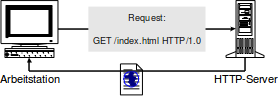
\includegraphics[width=0.6\hsize]{chap01/request_reply_protocol}
  \caption{Request reply protocol.}
  \label{fig:request_reply_protocol}
\end{figure}

An important type of content transferred is HTML. It is the lingua
franca for publishing hypertext on the World Wide Web. It is a
non-proprietary format based upon SGML, and can be created and
processed by a wide range of tools, from simple plain text editors -
you type it in from scratch- to sophisticated WYSIWYG authoring tools.
HTML uses tags such as <h1> and </h1> to structure text into headings,
paragraphs, lists, hypertext links etc. 



